\section{Project description}

\subsection{Background}

Rydberg atoms are characterized by a single valence electron in a highly excited electronic bound state (with principal quantum number $n \gg 1$) \cite{Gallagher1994}. These atoms have exaggerated features, because many experimentally important properties scale as a high power of $n$: their physical size $a_\mathrm{Ry} \sim a_0 n^2$ (where $a_0$ is the Bohr radius), radiative lifetimes as $n^3$, the dipole-dipole interaction between different atoms as $n^4$. Their most widely used interaction is the Rydberg blockade \cite{Jaksch2000}, where an atom in the Rydberg state can suppress the excitation of physically nearby atoms. This interaction can be turned on and off with very good contrast (12 orders of magnitude in coupling strength). The above properties allow for very efficient coupling of Rydberg states and have many uses in quantum information and quantum simulation (such as the recently observed entanglement between Rydberg atoms \cite{Wilk2010}). Rydberg atomic systems were extensively studied in the last decade, both single atoms and Rydberg ensemble properties. A detailed discussion about the current state of research can be found in a recent review paper \cite{Saffman2010}.
%% Most of these experiments require sub-Doppler cooling and shielding from electromagnetic fields, since the Rydberg state is sensitive to shifts introduced by motion and external fields.

Another group of physical systems that is often compared to Rydberg atomic ensembles in terms of quantum computing potential is ion traps. They have a number of advantages, such as individual addressing of ions \cite{Nagerl1999}, fast and high fidelity quantum gates \cite{Benhelm2008}, very long storage and coherence times \cite{Lucas2007}. The coupling between ions is through the Coulomb interaction which allows strong coupling, but with the disadvantage that the interaction is always present. This makes many-qubit systems more prone to motional decoherence than the weakly interacting atomic ensembles, where the atom-atom interaction can efficiently turned off . The electronic structure of ions, however, is very close to those neutral atoms used in the Rydberg-type experiments, both having a single valence electron. It is then natural to ask how would ionic Rydberg systems behave?

A recent theoretical proposal \cite{Mueller2008} examined the possibility of Rydberg ions, and while they inherit many properties from both trapped ions and Rydberg atoms, they have qualitatively different interactions from both. This difference stems from the fact that the highly excited electron can be described as ``nearly free'', thus Rydberg ions in an ion trap behave as a composite system: a double-positively charged, heavy core and a highly delocalized electron (see Figure \ref{fig:iontrap}). In most experiments the atoms are well localized ($x_{ho}$ oscillator length is small), and size of the atom (the extent of the highly excited electron) $a_\mathrm{Ry}$ is smaller than the inter-ionic distance $\xi$. Under these conditions the interaction between the ground state ions, Rydberg ions and the electromagnetic field of the trap can be described as a combination of charge-charge, charge-dipole, charge-quadrupole and dipole-dipole interaction (while trapped ions only exhibit the first, Rydberg atoms the last contribution). Many of these interactions are externally tunable by the trap electric field strength or by the choice of the Rydberg level $n$. Their combination makes possible to potentially create many different coupling schemes. Based on the proposals of \cite{Mueller2008} Rydberg ions can have stronger interaction than either neutral atoms or ions in conventional ion traps, which enables faster quantum gate operation. Recent results of fast entangling operation of ion qubits with optical frequency combs \cite{Hayes2010} suggests that similar technique could also be used to speed up Rydberg ion manipulation.

\begin{figure}
  \begin{center}
    \includegraphics[width=0.7\textwidth]{iontrap}
    \caption{Adapted from \cite{Mueller2008}, the schematic view of Rydberg ions in an ion trap, where $x_{ho}$ is the oscillator length of the ion core, $a_\mathrm{Ry}$ is the size of the Rydberg orbit, $\xi$ is the ion-ion separation. Typical experiments would have $x_{ho} \ll a_\mathrm{Ry} \ll \xi$ with $\xi \approx 5 \mu\mathrm{m}$.}
  \end{center}
  \label{fig:iontrap}
\end{figure}

These properties hint at the wide variety of uses for Rydberg ions. On one hand they can become part of the standard trapped ion toolbox by providing fast and high fidelity quantum gates. Alternatively they can become resources themselves for quantum information processing, and also, by means of the Rydberg blockade scheme, for simulation of interacting spin-systems. Combining either path with previous techniques would open up new avenues for experiments. Given my experience with designing and implementing ion trap systems, I plan to lead a research program exploring and utilizing this new type of atomic system.

Given the requirements for energy level separations, radiative lifetimes, existence of metastable-states, presence or absence of hyperfine structure, the best candidate ion species are Ca$^+$, Yb$^+$, Ba$^+$.

\subsection{Research objectives}
The research objectives of this proposal are the following:
\begin{enumerate}
 \item Build up an ion trap experiment based on a species that is selected based on its qualities for Rydberg ion.
 \item Build up the mixed microwave \& laser system that was theoretically proposed \cite{Mueller2008} to demonstrate Rydberg ion creation and then single-qubit manipulation.
 \item Demonstrate Rydberg blockade in the ion system, thus setting the way for two-qubit gates and entanglement.
 \item Mixed ion species for sympathetic cooling \cite{Home2009} or selective excitation of qubits.
 \item Mixed ground state ion Rydberg ion quantum computing, where ground state ions are for information storage and transport, Rydberg-type interaction implements fast gates.
 \item Implement quasi-1D Ising spin chain \cite{Olmos2009} in a ring trap geometry \cite{Champenois2010}.
 \item Parallel to the experimental effort, establish solid theoretical background for these systems, thus searching for other possible single- and two-ion manipulation methods.
\end{enumerate}
